\documentclass[aspectratio=169,10pt]{beamer}
\usepackage{beamerthemencsu}
\usepackage{graphicx,booktabs,tikz}
\usetikzlibrary{positioning}
\title{Verifier-Supervised Look-Back}
\subtitle{Teaching a phone agent which screen to re-read, without labelling anything}
\author{Mingshuo Wang}
\institute{North Carolina State University}
\date{}

\newcommand{\bigstat}[3]{{\color{#1}\textbf{#2}}\;{\footnotesize\color{ncgray}#3}}

\begin{document}

% ---------- 1. title: brand says start with red ----------
{\setbeamercolor{background canvas}{bg=wolfred}
\begin{frame}[plain]
\vspace{1.1cm}
{\color{white}\LARGE\bfseries Verifier-Supervised Look-Back\par}
\vspace{0.35cm}
{\color{white}\large Teaching a phone agent which screen to re-read,\\without labelling anything\par}
\vspace{1.0cm}
{\color{white}\normalsize Mingshuo Wang\par}
{\color{white!80!wolfred}\small North Carolina State University\par}
\vspace{0.5cm}
{\color{white!80!wolfred}\scriptsize github.com/WMSlalalala/verifier-supervised-lookback\par}
\end{frame}}

% ---------- 2. what a phone agent does ----------
\begin{frame}{A phone agent does what you would do, one screen at a time}
\vspace{0.1cm}
\begin{columns}[T]
\begin{column}{0.56\textwidth}
\vspace{0.4cm}
\begin{itemize}\setlength\itemsep{0.55em}
\item It is given a task in plain English.
\item It sees \alert{one screen}, picks \alert{one action}: tap, scroll, or type.
\item The screen changes. Repeat.
\end{itemize}
\vspace{0.7cm}
{\color{ncgray}A long task runs 15--30 screens and crosses several apps.}
\end{column}
\begin{column}{0.42\textwidth}
\centering
\begin{tikzpicture}[node distance=3mm,every node/.style={font=\scriptsize}]
\node[draw=ncgray,rounded corners,minimum width=2.6cm,minimum height=0.75cm,align=center] (a) {screen};
\node[draw=wolfred,very thick,rounded corners,minimum width=2.6cm,minimum height=0.75cm,below=of a,align=center,fill=red!4] (b) {the agent picks\\an action};
\node[draw=ncgray,rounded corners,minimum width=2.6cm,minimum height=0.75cm,below=of b,align=center] (c) {new screen};
\draw[-latex,ncgray] (a)--(b); \draw[-latex,ncgray] (b)--(c);
\draw[-latex,wolfred,thick] (c.east) -- ++(0.7,0) |- (a.east);
\end{tikzpicture}
\end{column}
\end{columns}
\end{frame}

% ---------- 3. THE PROBLEM (real screenshots) ----------
\begin{frame}{Sometimes the answer left the screen a long time ago}
\vspace{-0.15cm}
\centering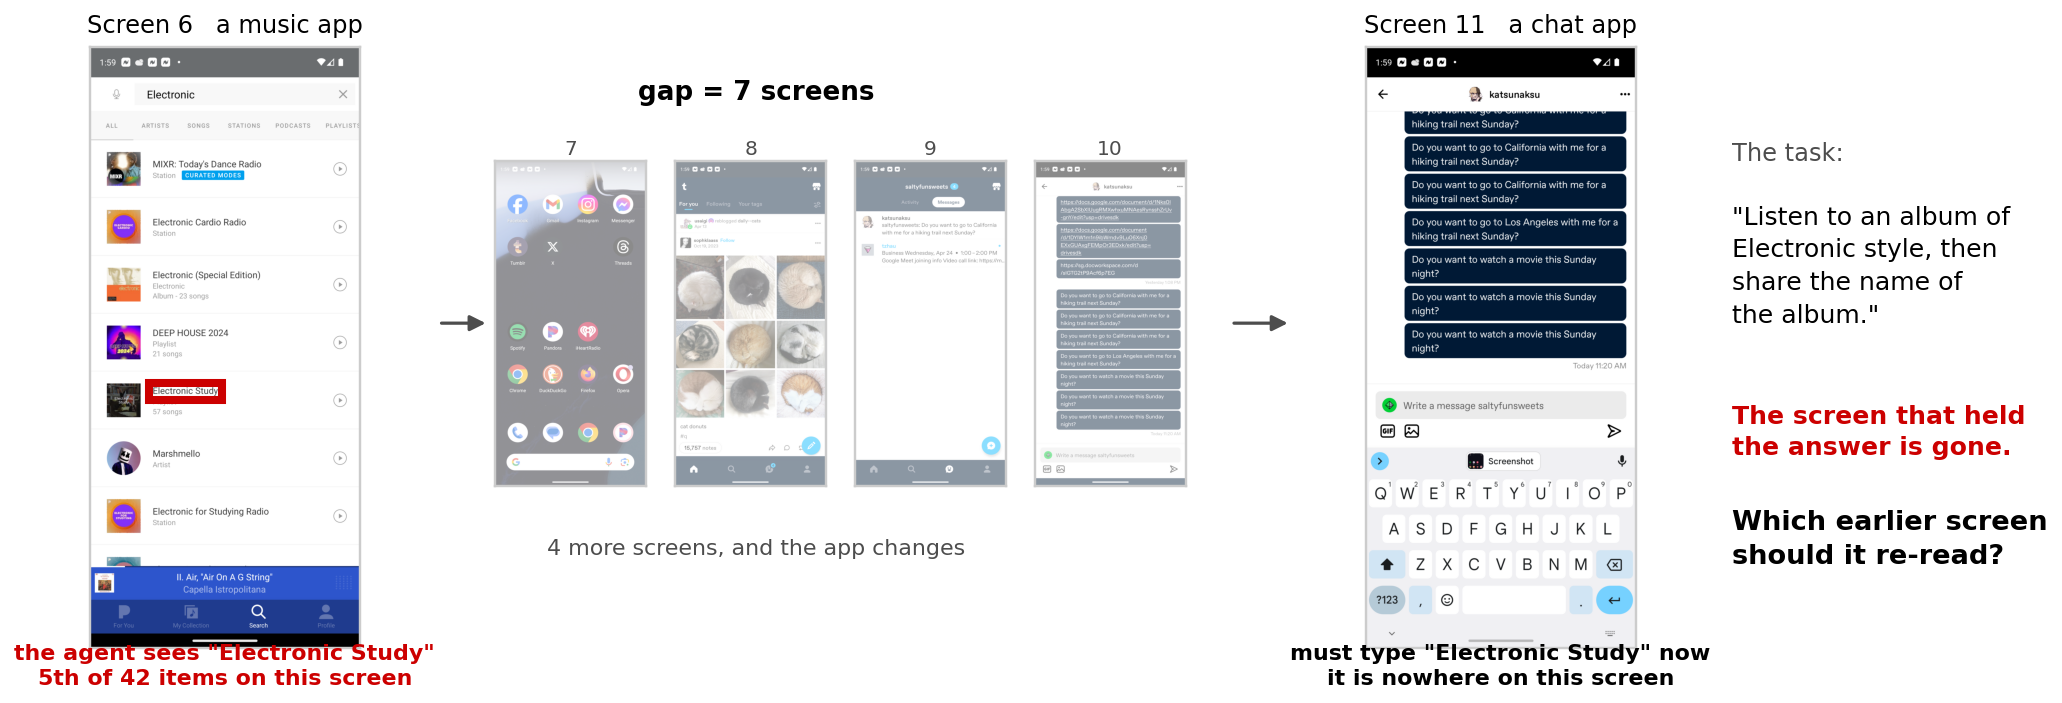
\includegraphics[width=0.99\textwidth]{figures/problem.png}
\end{frame}

% ---------- 4. how common ----------
\begin{frame}{This is not a corner case, but the usual benchmarks hide it}
\vspace{0.35cm}
\centering
\begin{tabular}{lrrr}
\toprule
& tasks & avg.\ length & tasks needing an old screen \\
\midrule
AITZ {\footnotesize(a common benchmark)} & 2,504 & 7.4 screens & \bigstat{ncgray}{0}{of 18,643 steps} \\[0.25em]
GUI-Odyssey {\footnotesize(long, cross-app)} & 7,735 & 15.4 screens & \bigstat{wolfred}{31\%}{of sampled tasks} \\
\bottomrule
\end{tabular}
\vspace{0.9cm}
\begin{itemize}
\item Short benchmarks cannot contain the problem: the task ends before the gap opens.
\item When it does happen, the answer sits \alert{13th of 33 items} on its screen, never first.
\end{itemize}
\end{frame}

% ---------- 5. two options, and the wall ----------
\begin{frame}{Two obvious options, and why neither is trained}
\vspace{0.3cm}
\begin{columns}[T]
\begin{column}{0.48\textwidth}
{\large\bfseries 1. Keep everything}\\[0.4em]
{\color{ncgray}Put the text of every past screen into the prompt.}\\[0.6em]
Finds the right screen \textbf{68\%} of the time early in a task,\\ \alert{46\%} late in a task.
\end{column}
\begin{column}{0.48\textwidth}
{\large\bfseries 2. Keep a one-line index}\\[0.4em]
{\color{ncgray}Write one short line per screen, pick a line, re-read that screen.}\\[0.6em]
Finds it \alert{41\%} of the time.
\end{column}
\end{columns}
\vspace{0.9cm}
\hrule
\vspace{0.5cm}
\centering
{\large Both are \alert{prompted}, never trained.}\\[0.4em]
{\color{ncgray}Training needs someone to say which earlier screen was the right one.\\
The one system that did train this way paid for 8{,}600 hand-written labels.}
\end{frame}

% ---------- 6. THE IDEA ----------
\begin{frame}{The idea: the labels are already there}
\vspace{-0.1cm}
\centering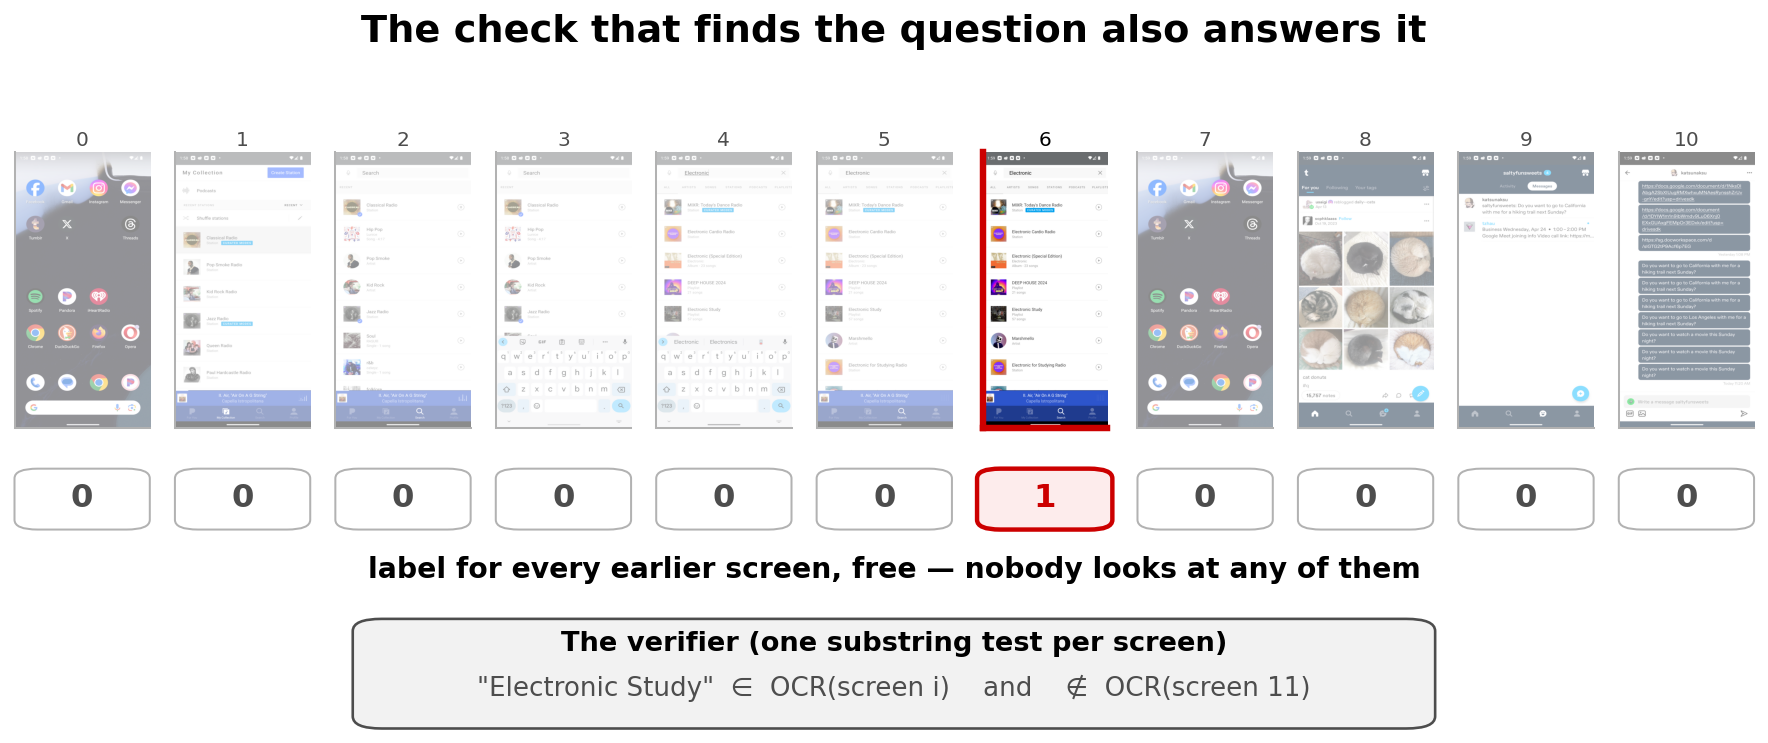
\includegraphics[width=0.96\textwidth]{figures/idea.png}
\end{frame}

% ---------- 7. two models ----------
\begin{frame}{Same free labels, two ways to use them}
\vspace{0.5cm}
\begin{columns}[T]
\begin{column}{0.47\textwidth}
\begin{block}{}
{\color{ncaqua}\large\bfseries Read the whole history}\\[0.5em]
One call. All past screens in the prompt.\\ Output: a screen number.\\[0.5em]
{\color{ncgray}188 training examples}
\end{block}
\end{column}
\begin{column}{0.47\textwidth}
\begin{block}{}
{\color{wolfred}\large\bfseries Score each screen alone}\\[0.5em]
One call \emph{per screen}. Output: the chance this screen holds the answer. Take the highest.\\[0.5em]
{\color{ncgray}2,861 training examples}
\end{block}
\end{column}
\end{columns}
\vspace{0.8cm}
\centering{\color{ncgray}Same 7B model, same LoRA adapter, same labels. The only difference is how the history reaches it.}
\end{frame}

% ---------- 8. main result ----------
\begin{frame}{What the free labels buy}
\vspace{-0.1cm}
\centering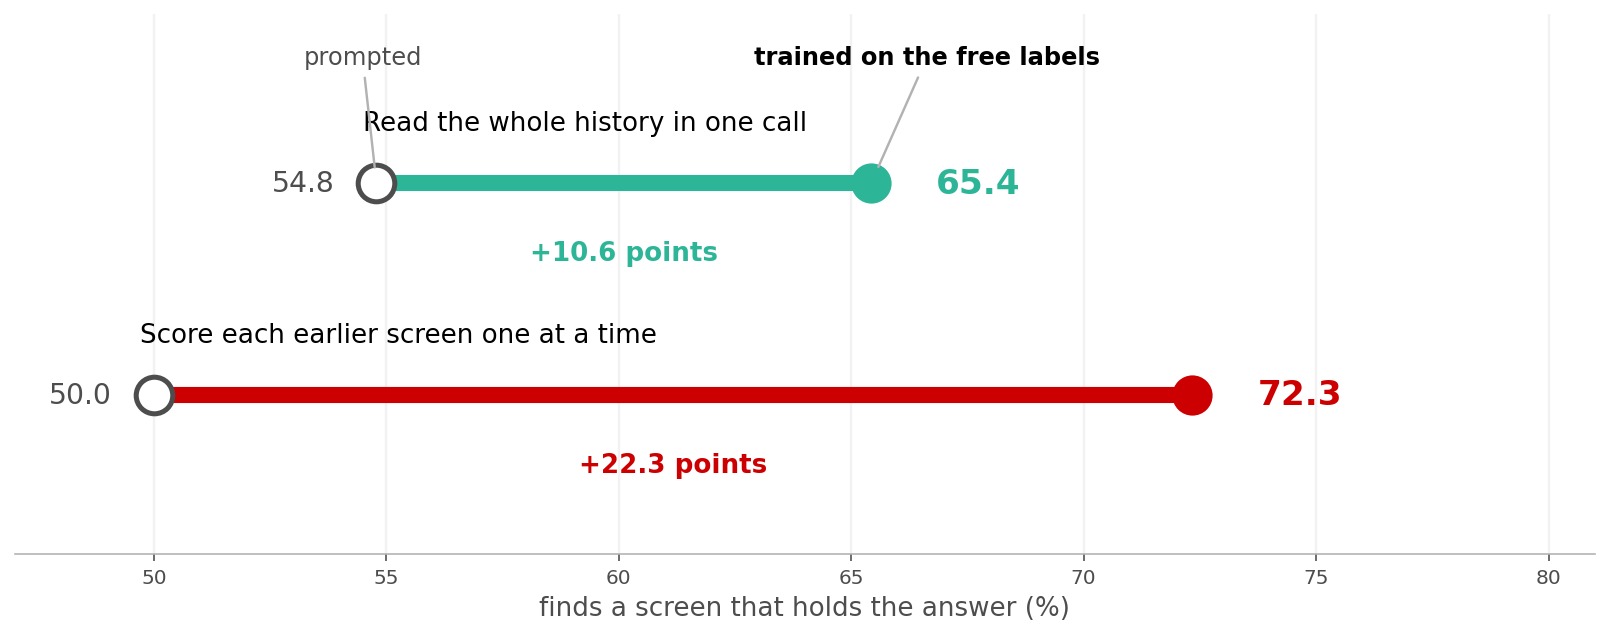
\includegraphics[width=0.84\textwidth]{figures/labels_buy.png}
\vspace{-0.2cm}
\begin{center}
{\large The labels help \alert{both}. Which architecture wins is \alert{not} statistically separable ($p=0.086$).}
\end{center}
\end{frame}

% ---------- 9. by gap ----------
\begin{frame}{Scoring one screen at a time helps in one specific place}
\vspace{-0.1cm}
\centering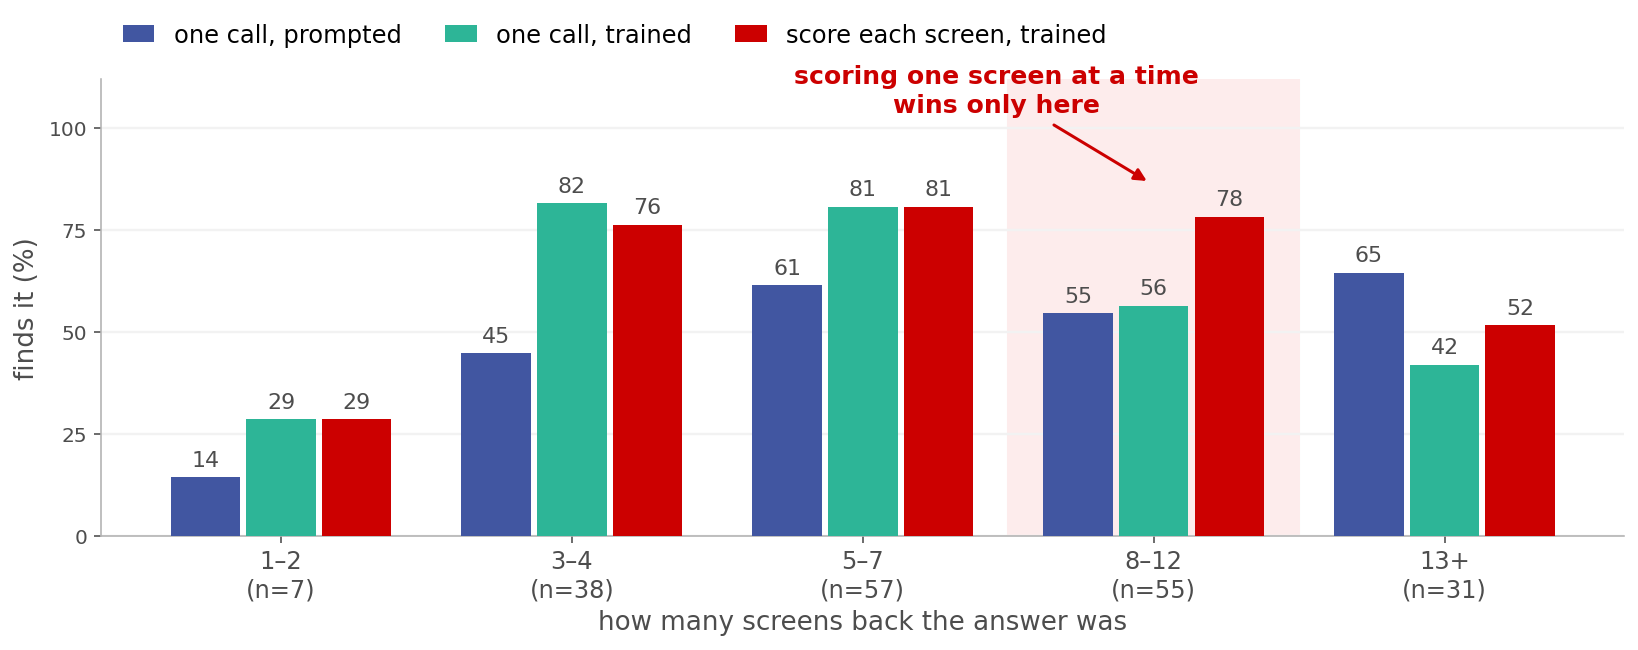
\includegraphics[width=0.88\textwidth]{figures/by_gap.png}
\vspace{-0.1cm}
\begin{center}{\color{ncgray}8--12 screens back is where one call has a dozen look-alike candidates to weigh at once.}\end{center}
\end{frame}

% ---------- 10. external ----------
\begin{frame}{Checked once on data no design decision ever saw}
\vspace{0.1cm}
\centering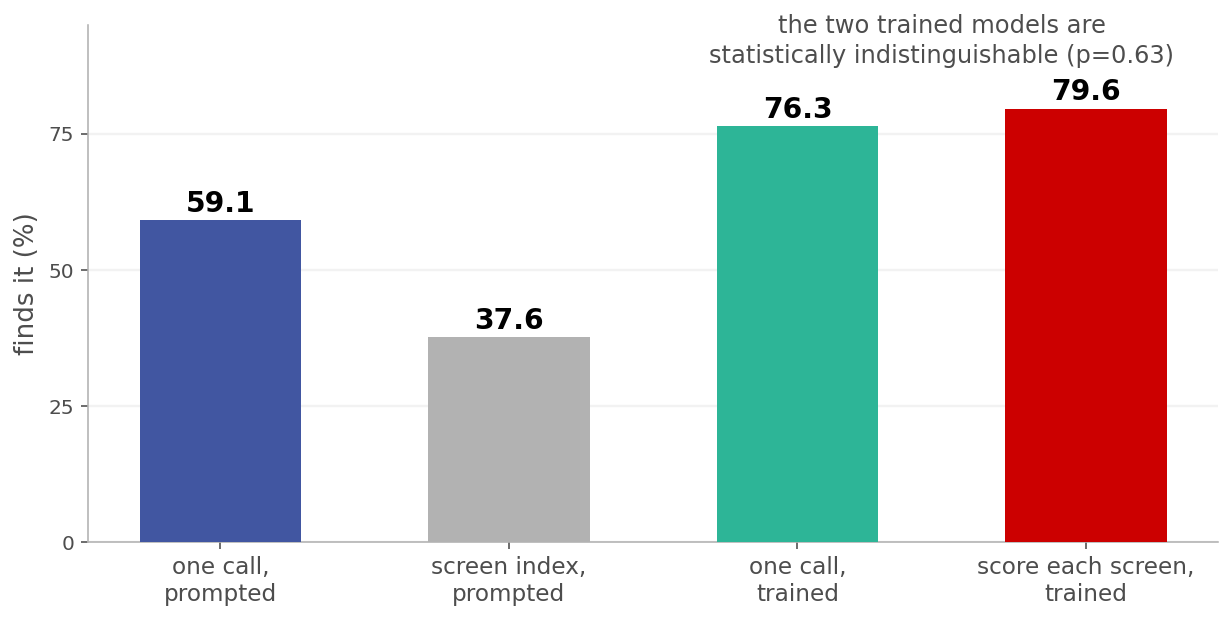
\includegraphics[width=0.66\textwidth]{figures/external.png}
\vspace{0.1cm}
\begin{center}
{\color{ncgray}93 cases from a fourth batch of 400 trajectories, mined after everything was frozen.}
\end{center}
\end{frame}

% ---------- 11. what failed ----------
\begin{frame}{What did not work}
\vspace{0.45cm}
\begin{itemize}\setlength\itemsep{0.8em}
\item \textbf{Very old screens (13+ back).} Both trained models drop \alert{below} the untrained baseline. They learn that the answer is usually 5 screens back, and that prior misfires at the tail.
\item \textbf{The one-line index.} Five ways of training or re-prompting its writer: none passes plain full history. An oracle that hand-picks the best line reaches full-history level and no higher.
\item \textbf{A shortcut that looked great.} A rule that just re-reads the two previous screens beat everything by 17 points, until I found the bug that made it work.
\end{itemize}
\end{frame}

% ---------- 12. the trap ----------
\begin{frame}{The bug worth telling you about}
\vspace{0.4cm}
\begin{columns}[T]
\begin{column}{0.52\textwidth}
My first mining rule asked:\\[0.4em]
{\color{ncgray}\itshape is the typed text on an earlier screen?}\\[0.9em]
It should have asked:\\[0.4em]
{\color{wolfred}\itshape is it on an earlier screen \textbf{and not on the current one}?}
\end{column}
\begin{column}{0.44\textwidth}
\begin{block}{}
\centering
{\large\textbf{58\%}}\\{\footnotesize of my long-task cases needed \\ \alert{no memory at all}}
\end{block}
\end{column}
\end{columns}
\vspace{0.7cm}
\hrule
\vspace{0.45cm}
\centering
Before the fix: the shortcut wins by \textbf{17 points}.\quad After: it loses by \textbf{23}.\\[0.3em]
{\color{ncgray}The filter changed the conclusion more than any method I tried.}
\end{frame}

% ---------- 13. takeaway: brand says end with red ----------
{\setbeamercolor{background canvas}{bg=wolfred}
\begin{frame}[plain]
\vspace{0.8cm}
{\color{white}\Large\bfseries Takeaway\par}
\vspace{0.7cm}
{\color{white}\large
The test that \emph{finds} this problem also \emph{labels} it.\par
\vspace{0.5em}
That free supervision is what works --- not the architecture I bet on.\par}
\vspace{1.0cm}
{\color{white!85!wolfred}\normalsize
$+10.6$ and $+22.3$ points from labels nobody wrote\\[0.3em]
the two trained models are indistinguishable\\[0.3em]
13+ screens back is still open\par}
\vspace{0.8cm}
{\color{white!80!wolfred}\small github.com/WMSlalalala/verifier-supervised-lookback\par}
\end{frame}}

\end{document}
